\chapter{Tabela de Probabilidades - Distribuição Normal Padrão}

\begin{figure}[h]
	\center
	\label{fig:tab-prob-normal-padrao}
	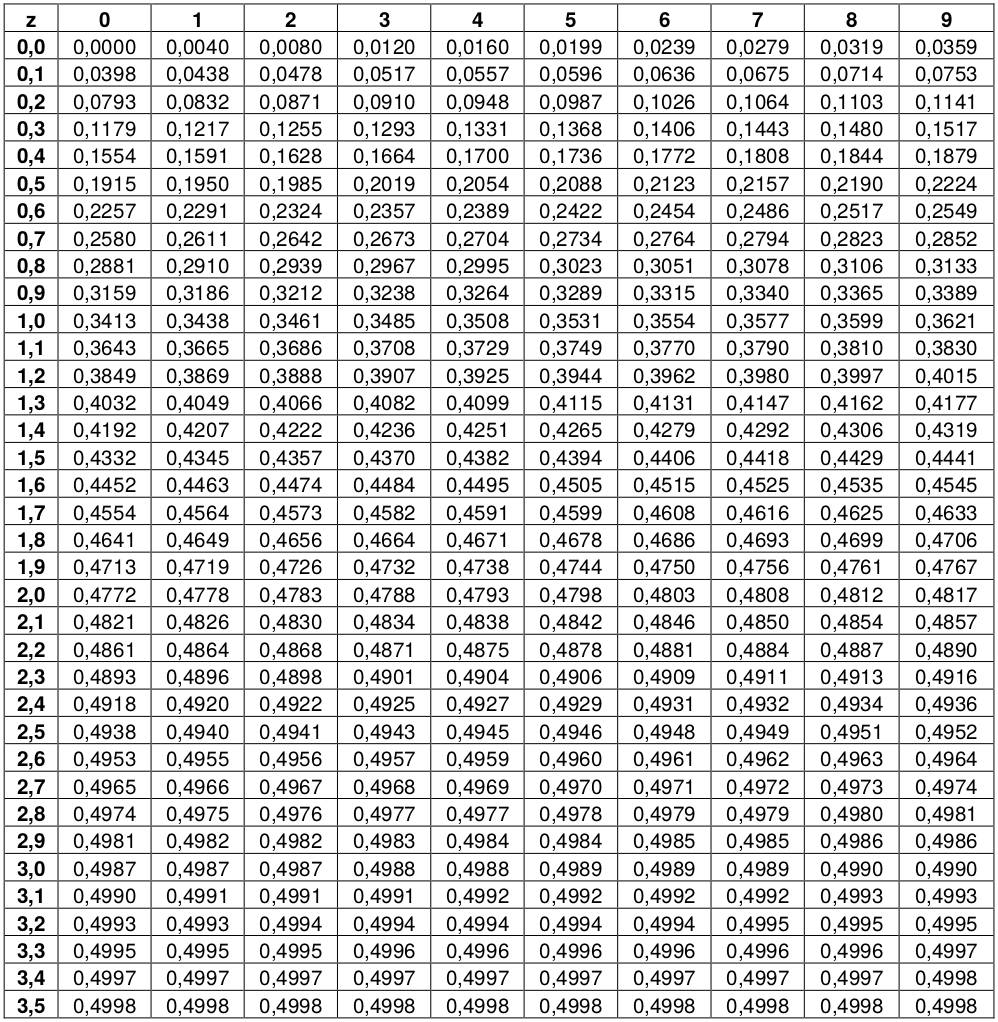
\includegraphics[scale=2]{apendices/prob-normal-padrao.png}
\end{figure}

Onde:
\begin{itemize}
	\item O valores de \(z\) estão nos cabeçalhos de linha e coluna;
	\item As probabilidades estão no centro.
\end{itemize}

